
%%%%%%%%%%%%%%%%                                ~~~~~~~~~~~~~~~~~~~~~~~~~~~~~~~~~~~~~~~~~~~~~~~~~~
% CONDITIONALS %
%%%%%%%%%%%%%%%%                                ~~~~~~~~~~~~~~~~~~~~~~~~~~~~~~~~~~~~~~~~~~~~~~~~~~

\newif\ifPeerReview\PeerReviewfalse              % Whether to create the PeerReview version or
                                                % Journal version
\newif\ifOnlineColor\OnlineColortrue            % Compile online color version?

\newif\ifFlatArchive\FlatArchivefalse           % Whether archive is flat (messy) or contain 
                                                % subfolders for graphics etc.
\newif\ifFloatAtEnd\FloatAtEndfalse             % Available in PeerReview mode:
                                                % Place floats at end of document?
\newif\ifTODO\TODOtrue                        % Use todo notes?

\ifOnlineColor
   \newcommand\figPostfix{_online}              % Colored images online
\else
   \newcommand\figPostfix{_bw}                  % Black and white in journal
\fi

%%%%%%%%%%%%                                    ~~~~~~~~~~~~~~~~~~~~~~~~~~~~~~~~~~~~~~~~~~~~~~~~~~
% IEEEtran %
%%%%%%%%%%%%                                    ~~~~~~~~~~~~~~~~~~~~~~~~~~~~~~~~~~~~~~~~~~~~~~~~~~

\ifPeerReview
\documentclass[10pt,journal,draftclsnofoot,onecolumn]{IEEEtran}
% \newcommand\CLASSINPUTbaselinestretch{1.66}     % http://theoval.cmp.uea.ac.uk/~nlct/latex/thesis/node17.html
\else
\documentclass[journal]{IEEEtran}
\fi

% \RequirePackage[latin1]{inputenc}%              % Set input encoding (optionally latin1)
% \RequirePackage[T1]{fontenc}%                 % Set font encoding
% \usepackage[norsk]{babel}

% Single column review mode:
%\documentclass[12pt,journal,onecolumn]{IEEEtran}
%\newcommand\CLASSINPUTbaselinestretch{2}
%\RequirePackage{calc}
%\RequirePackage{fp} 
% Left margin = 1 inch + hoffset + oddsidemargin (or evensidemargin)
% Adding the 2cm gutter width to the odd/even side margins:
%\setlength\hoffset{0pt}
%\setlength\oddsidemargin{4cm}       % 4cm margins on the left side
%\addtolength\oddsidemargin{-1in}    % Subtract the initial 1 inch
%\setlength\textwidth{21cm-8cm}    % A4 width (21cm) minus margins on either side

%%%%%%%%%%%%%%%%%%%%%%%%%%%%%%                  ~~~~~~~~~~~~~~~~~~~~~~~~~~~~~~~~~~~~~~~~~~~~~~~~~~
% IEEE ''APPROVED'' PACKAGES %
%%%%%%%%%%%%%%%%%%%%%%%%%%%%%%                  ~~~~~~~~~~~~~~~~~~~~~~~~~~~~~~~~~~~~~~~~~~~~~~~~~~

\usepackage{cite}

\ifCLASSINFOpdf
   \usepackage[dvips]{graphicx}                 % Might not work. Use 'latex' instead of 
   \ifFlatArchive\else                          % 'pdflatex'
      \graphicspath{./gfx/}
   \fi
\else
   \usepackage[dvips]{graphicx}
   \ifFlatArchive\else
      \graphicspath{./gfx/}
   \fi
\fi

\RequirePackage[table,dvipsnames,svgnames]{xcolor}

\usepackage[cmex10]{amsmath}                    % cmex10 option to be IEEE explore compliant
\interdisplaylinepenalty=2500                   % Allows multiline equations to be broken

% \RequirePackage{amssymb}

\RequirePackage{array}

% \ifCLASSOPTIONcompsoc
%    \usepackage[caption=false,font=normalsize,labelfont=sf,textfont=sf]{subfig}
% \else
%    \usepackage[caption=false,font=footnotesize]{subfig}
% \fi

% \usepackage{caption}
% \usepackage{subcaption}
\usepackage{color}
\usepackage{calc}
\usepackage{fp}

% 
% \ifCLASSOPTIONcaptionsoff                       % IEEE promoted hack to turn off captions from the 
%    \let\MYorigsubfloat\subfloat                 % subfloat package should the captionsoff option
%    \renewcommand{\subfloat}[2][\relax]{\MYorigsubfloat[]{#2}} % be specified.
% \fi

\ifFloatAtEnd
\ifCLASSOPTIONcaptionsoff                       % Places float at the end of the document when the
  \usepackage[nomarkers]{endfloat}              % captionsoff options is specified to IEEEtrans.cls
  \let\MYoriglatexcaption\caption               % (PeerReview mode)
  \renewcommand{\caption}[2][\relax]{\MYoriglatexcaption[#2]{#2}}
\fi
\fi

\usepackage{fixltx2e}                           % Fix some twocolumn float problems

\usepackage{stfloats}                          % Allows: \begin{figure*}[!b]
                                                % (double column figures on top/bottom)

\usepackage{url}                                % Support for handling and breaking URLs

% NOTE: PDF hyperlink and bookmark features are not required in IEEE
%       papers and their use requires extra complexity and work.
\newcommand\MYhyperrefoptions{bookmarks=true,bookmarksnumbered=true,
pdfpagemode={UseOutlines},plainpages=false,pdfpagelabels=true,
colorlinks=true,linkcolor={black},citecolor={black},urlcolor={black},
pdftitle={A Fast GPU Sonar Simulator for Automatic Target Recognition},
pdfsubject={},
pdfauthor={Jo Inge Buskenes},
pdfkeywords={adaptive beamforming, beamforming, complexity, sonar, active}}%
\ifCLASSINFOpdf
   \usepackage[\MYhyperrefoptions,pdftex]{hyperref}
\else
   \usepackage[\MYhyperrefoptions,breaklinks=true,dvips]{hyperref}
   \usepackage{breakurl}                        % Allows 'dvips' driver to break links
\fi

%%%%%%%%%%%%%%%%%%%%%%%                         ~~~~~~~~~~~~~~~~~~~~~~~~~~~~~~~~~~~~~~~~~~~~~~~~~~
% ADDITIONAL PACKAGES %       
%%%%%%%%%%%%%%%%%%%%%%%                         ~~~~~~~~~~~~~~~~~~~~~~~~~~~~~~~~~~~~~~~~~~~~~~~~~~

% \ifPeerReview
% \let\OldIncludegraphics{\includegraphics}
% \usepackage{letltxmacro}
% \LetLtxMacro{\OldIncludegrsaphics}{\includegraphics}
% \renewcommand{\includegraphics}[2][]{\OldIncludegraphics[width=\linewidth, #1]{#2}}
% \fi

% % \makeatletter
% % \def\maxwidth{\ifdim\Gin@nat@width>\linewidth\linewidth
% % \else\Gin@nat@width\fi}
% % \makeatother
% % \let\Oldincludegraphics\includegraphics
% % \renewcommand{\includegraphics}[1]{\Oldincludegraphics[width=\maxwidth]{#1}}

% \usepackage[maxfloats=40]{morefloats}
\newcounter{todoidx}
% \setcounter{todoidx}

\ifTODO
   \definecolor{todobackground}{rgb}{0.95,0.95,0.95}
   \setlength\marginparsep{1pt}
   \setlength\marginparwidth{35pt}
   \newlength\marginparwidthsmall
   \setlength\marginparwidthsmall{\marginparwidth}
   \addtolength\marginparwidthsmall{-7pt}
   \newcommand\todo[1]{%
      \addtocounter{todoidx}{1}%
      {\color{Red}\bf(\thetodoidx{})}%%\fbox{\bf\thetodoidx{}}}%
      \marginpar{%
         {\vspace*{-10pt}\color{Red}\fbox{\bf\thetodoidx{}}}\\%
         \fcolorbox{red}{todobackground}{\parbox{\marginparwidthsmall}{\scriptsize #1}}}}

   \newcommand\todopar[1]{\fcolorbox{red}{white}{\parbox{0.97\linewidth}{#1}}}
\else
%    \usepackage[disable]{./todonotes} 
   \newcommand\todo[1]{}
\fi

\newenvironment{narrow}[2]{%
\begin{list}{}{%
\setlength{\topsep}{0pt}%
\setlength{\leftmargin}{#1}%
\setlength{\rightmargin}{#2}%
\setlength{\listparindent}{\parindent}%
\setlength{\itemindent}{\parindent}%
\setlength{\parsep}{\parskip}}%
\item[]}{\end{list}}

\usepackage{float}

\ifOnlineColor
   \definecolor{tabBlue}{HTML}{AACCFF}
\else
   \definecolor{tabBlue}{HTML}{CCCCCC}
\fi

%%%%%%%%%%                                      ~~~~~~~~~~~~~~~~~~~~~~~~~~~~~~~~~~~~~~~~~~~~~~~~~~
% MACROS %       
%%%%%%%%%%                                      ~~~~~~~~~~~~~~~~~~~~~~~~~~~~~~~~~~~~~~~~~~~~~~~~~~

\newcommand\graphicsAI[2][]{%
  \immediate\write18{./bin/laFigure #2 #1}%
  \input{result}}%
  
% \DeclareMathOperator*{\argmin}{\text{arg}\;\text{min}}

\newcommand\Fig[1]{Fig.~\ref{#1}}

\newcommand\Grey[1]{{\color{Grey}#1}}
\newcommand\Red[1]{{\color{Red}#1}}
\newcommand\Blue[1]{{\color{Blue}#1}}
\newcommand\DarkBlue[1]{{\color{DarkBlue}#1}}
\newcommand\LightBlue[1]{{\color{LightBlue}#1}}
\newcommand\Brown[1]{{\color{Brown}#1}}
\newcommand\Green[1]{{\color{Green}#1}}
\newcommand\SeaGreen[1]{{\color{SeaGreen}#1}}
\newcommand\Yellow[1]{{\color{yellow}#1}}
\newcommand\Orange[1]{{\color{orange}#1}}

\newcommand\nn{\nonumber\\}

\newcommand\nmat[1]{\begin{matrix}#1\end{matrix}}
\newcommand\bmat[1]{\begin{bmatrix}#1\end{bmatrix}}
\newcommand\case[1]{\begin{cases}#1\end{cases}}
\newcommand\textbox[2]{\footnotesize\text{\parbox{#1}{\centering\emph{#2}}}}

\newcommand\rand{\text{rand}}
\newcommand\randn{\text{randn}}
\newcommand\rect{\text{rect}}
\newcommand\sinc{\text{sinc}}
\newcommand\tr{\text{tr}}
\newcommand\adj{\text{adj}}

% \newcommand\max{\text{max}}
\newcommand\argmin[1]{\text{arg}\;\underset{#1}{\text{min}}}

\newcommand\qqquad{\quad\qquad}
\newcommand\qqqquad{\qquad\qquad}

% \renewcommand\l[1]{\left#1}
% \renewcommand\r[1]{\right#1}

% {\text{\parbox{1.5cm}{\centering volume hyper- sphere}}}

%Keyword colouring:
\newcommand\kw[1]{#1}
\newcommand\parm[1]{#1}%\color{Black}#1\color{Black}}

\newcommand\of[1]{\scriptstyle(\parm{#1})\displaystyle}
\newcommand\df[1]{\scriptstyle[\parm{#1}]\displaystyle}
\newcommand\var[3]{#1_\text{#2}\of{#3}}

\newcommand\diag{\text{diag}}

% \raisebox{lift}[extend-above-baseline][extend-below-baseline]{text}
\newcommand\mt[1]{\text{\emph{#1}}} %mt = mathtext
\newcommand\mathnorm{\textstyle}
\newcommand\mathbig[1]{\displaystyle#1\mathnorm}
\newcommand\mathsmall[1]{\scriptstyle#1\mathnorm}
\newcommand\mathtiny[1]{\scriptscriptstyle#1\mathnorm}
\newcommand\sfrac[2]{\scriptstyle\raisebox{0.25pt}[0pt][0pt]{$\frac{#1}{#2}$}\mathnorm}
\newcommand\nfrac[2]{\textstyle\frac{#1}{#2}\displaystyle}

\newcommand\sumu[1]{\sum\limits^{#1}\;}
\newcommand\suml[1]{\sum\limits_{#1}\;}
\newcommand\sumb[2]{\sum\limits_{#1}^{#2}\;}

\newcommand\produ[1]{\prod\limits^{#1}\;}
\newcommand\prodl[1]{\prod\limits_{#1}\;}
\newcommand\prodb[2]{\prod\limits_{#1}^{#2}\;}

\newcommand\defeq{\overset{\underset{\mathrm{def}}{}}{=}}

%Math macros:
\newcommand\T{^{\scriptscriptstyle T}}
\renewcommand\H{^{\scriptscriptstyle H}}

\renewcommand\vec[1]{\boldsymbol{#1}}
\newcommand\mat[1]{\boldsymbol{#1}}

\newcommand\Om{O_\text{m}}
\newcommand\Oa{O_\text{a}}
\newcommand\Nl{N_\text{l}}
\newcommand\Nk{N_\text{k}}
\newcommand\1{\vec 1}
\newcommand\I{\mat I}
\renewcommand*\a{\vec a}
\newcommand*\f{\vec f}
\renewcommand*\i{\vec i}
\renewcommand*\k{\vec k}
\newcommand*\n{\vec n}
\newcommand*\p{\vec p}
\newcommand*\s{\vec s}
\newcommand*\w{\vec w}
\newcommand*\x{\vec x}
\newcommand*\y{\vec y}

\newcommand*\A{\mat A}
\newcommand*\B{\mat B}
\newcommand*\C{\mat C}
\newcommand*\E{\mat E}
\renewcommand*\P{\mat P}
\newcommand*\eP{\mat{\hat P}}
\newcommand*\R{\mat R}
\newcommand*\Ri{\R^{-1}}
\newcommand*\eR{\mat{\hat R}}
\newcommand*\eRi{\hat{\mat R}\;\!^{-1}}
\newcommand*\Navg{N_\text{avg}}
\newcommand*\W{\mat W}
\newcommand*\X{\mat X}
\newcommand*\Xd{\X_{\!\Delta}}
\newcommand*\Y{\mat Y}

\renewcommand\argmin{\text{argmin}}


\renewcommand*\P{\mat P}
\newcommand*\V{\mat V}
\newcommand*\M{\mat M}

\renewcommand*\L{\mat \Lambda}
\newcommand*\U{\mat U}
% \renewcommand*\t{\mathtiny{^T}}
% \newcommand*\h{\mathtiny{^H}}
\renewcommand*\t{^T}
\newcommand*\h{^H}

\usepackage{tikz}
\usetikzlibrary{shapes,snakes}
\usepackage{amsmath,amssymb}
% \usepackage{datatool}
% \usepackage{glossaries}

\newenvironment{outline}
{\begin{itemize}}
{\end{itemize}}



\begin{document}

\title{Low Complexity Adaptive Beamformer\\ for Active Sonar Imaging}

\author{Jo~Inge~Buskenes, %
        Andreas~Austeng, %
        Carl-Inge~Columbo~Nilsen%
\IEEEcompsocitemizethanks{\IEEEcompsocthanksitem All authors are with the Department
of Informatics, University of Oslo, Norway.}% <-this % stops a space

% \thanks{Manuscript received April 19, 2005; revised January 11, 2007.}
}

% The paper headers
\markboth{IEEE Journal of Oceanic Engineering}%
{Low Complexity Adaptive Beamformer for Active Sonar Imaging}

% Publishers ID mark:
%\IEEEpubid{0000--0000/00\$00.00~\copyright~2007 IEEE}

% use for special paper notices
%\IEEEspecialpapernotice{(Invited Paper)}

% for Computer Society papers, we must declare the abstract and index terms
% PRIOR to the title within the \IEEEcompsoctitleabstractindextext IEEEtran
% command as these need to go into the title area created by \maketitle.
\IEEEcompsoctitleabstractindextext{%
\begin{abstract}
\color{gray}

% 
% \begin{itemize}
% \item Dynamic weights $\Rightarrow$ greater contrast/resolution potential
% \item But:
% \begin{itemize}
% \item Active system $\Rightarrow$ noise and signal correlated $\Rightarrow$ adaptive beamformers no longer robust.
% \item Subarray averaging decorrelate the noise, but in the process we sacrifice resolution.
% \item Computationally complex O($M^3$) due to inversion of a spatial covariance matrix. LCA is only O($MW$). Even if Capon subspace/beamspace versions exist, they remain more complex than the LCA, and is not as ideally suited for implementation of SIMD hardware (GPUs, DSPs, ...).
% \end{itemize}
% \item LCA is inherently robust, is ``parameter free'' once setup with a well designed window set, and can often be implemented with minor modifications to already existing DAS beamformers.
% 
% The angular resolution and contrast in active sonar images depend on the beamformer's ability to receive signals from directions of interest, while suppressing noise and interference emanating from other directions. For sonar arrays, this is achieved by applying weights to the array channels.
% 
% While classical beamformers use predefined windows, adaptive beamformers estimate the optimal window by analytical evaluation of the data. The minimum variance (MV) beamformer, for instance, calculates the set of weights that minimises the variance of the beamformer's output. 
% 
We have implemented a Low Complexity Adaptive (LCA) beamformer, which adaptively selects a window from a predefined set. The set is comprised of windows that are typical solutions found by the Minimum Variance method. The LCA beamformer was tested using simulated and experimental data from the Kongsberg Maritime HISAS 1030 sonar. On a simulated scene with speckle, highlight and shadow, the beamformer offered better lateral edge definition compared to the MV beamformer, and speckle intensity and shape comparable to DAS and MV beamformers. These results were verified by the experimental data.
% 
% An attactive trait of the LCA is its low computational complexity; while the MV beamformer is of O($M^3$), the LCA method is of O($MW$), with $M$ being the number of channels and $W$ the number of windows. We made the LCA perform like the MV method using a well designed set of 30 windows. Hence, unless the array is very small, the proposed method will perform like the MV beamformer or better, and at a fraction of the computational cost.

% \end{itemize}

\end{abstract}

% Keywords (normally not used for peer reviews)
\ifPeerReview\else
\begin{IEEEkeywords}\color{gray}
Beamforming, adaptive beamforming, MVDR, LCA, sonar, active, complexity.
\end{IEEEkeywords}
\fi}
% \fi

% make the title area
\maketitle

% This command fixes abstract positioning for compsoc articles:
\IEEEdisplaynotcompsoctitleabstractindextext

% (Optional) Add some extra info on cover page of peer review papers:
% \ifCLASSOPTIONpeerreview
% \begin{center} \bfseries EDICS Category: 3-BBND \end{center}
% \fi

% Insert page break and insert second title (peer review mode)
\IEEEpeerreviewmaketitle

\section{Introduction}

% - Nature and scope
% - Past work
% - Methods
% - Brief summary results
% - Brief conclusions 

\IEEEPARstart{T}{he} best adaptive sonars are found in nature. Bats, for instance, use a high frequency sonar to detect, identify and track prey with amazing precision in caves amongst a myriad of other bats. Human made sonars have little to no adaptibility when data is collected, but some methods have been investigated in the data post processing. Perhaps the most studied adaptive method for reconstructing a sonar image is the minimum variance distortionless response (MVDR) beamformer~\cite{Capon1969}. It computes the window that is optimal in the sense of suppressing noise as much as possible while under the restriction of  preserving the signal of interest.

In many cases MVDR can improve image contrast and resolution compared to conventional static methods~\cite{Blomberg2013,Blomberg2012a,Dursun2009,Lo2004}. However, the computational complexity of conventional beamformers are linear with the number of channels, O($M$), while MVDR is at O($M^3$). This makes MVDR impracticable and sometimes infeasible. We have shown in previous studies that MVDR's complexity can be reduced, as well as accelerated significantly using graphics computing units (GPUs)~\cite{Buskenes2014,Asen2013}, but there is a way to avoid it altogether while achieving similar performance.

This method is called the Low Complexity Adaptive (LCA) beamformer. It was first proposed by Synnev\aa{}g et. al. in clinical medical imaging~\cite{Synnevag2008}, who demonstrated its ability to obtain very similar results to MVDR. It does this by applying a set of predefined windows and selects the one that is best able to suppress noise. Since it uses the same optimisation criterion as MVDR, it may be considered a version of MVDR with a reduced window solution space. As we will demonstrate, this works well because a robust MVDR design tends to create windows that resembles slightly varied versions of conventional ones. 

Synnev\aa{}g used a window set comprised of rectangular, Kaiser and inverted Kaiser functions. Of these a specific Kaiser window were micro-steered. We limit our study to the use of variations of the parametric Kaiser-Harris window, since we observed neglible performance difference to using this function or any of the common trigonometric ones. The Kaiser windows are easy to compute, is fairly insensitive to coefficient inaccuracies, and can create windows with shapes spanning from rectangular to Gaussian.


In this work we investigate a few questions related to the LCA that remain unanswered. One is what window function we can use, and how many windows we will need. 

Another question is what it takes to achieve double the resolution.


Using the LCA beamformer results in increased robustness and improved edge definition compared to the MV and DAS beamformers.


We will show that when applied to experimental data, the weights chosen by a robustified MVDR yield responses that tend to be symmetric and steered within a fraction of the -3dB resolution of the respective window. Then we create Kaiser windows of different types, and with varying degree of steering, that combined form a discrete version of the MVDR solution space. 



This article is outlined as follows:

% This article is outlined as follows: In Section \ref{methods}, we introduce the concept of adaptive beamforming and provide details on the MVDR and LCA method. Then, in \ref{maptogpu}, we investigate the complexity issue, discuss means for reducing arithmetic complexity, and detail an implementation that makes efficient use of the GPU's parallel resources. The final design is assessed in Sections \ref{images_and_benchmarks} and \ref{discussion}, where we provide benchmarks, comparisons with similar CPU implementations, and measures of how efficiently our implementation makes use of the GPU's resources.

% - How much oversampling
% - How many parameters, how great a span.
% 
% - Experiementl data, Holmengraa/cross
% 
% - Note on efficiency.
% 
% 
% From our work with MVDR it 
% 
% 
% Traditionally beamformers were static, but as processors get more powerful so with the emergence of more processing power 


% 
% \section{Methods}
% 
% At heart of the image formation process is a technique called beamforming, which creates a focus point at the pixel of interest. It does this by applying a suitable set of delays and weights to the array elements, such that signals emanating from the pixel location are emphasized constructively, while noise and interference from other directions sum destructively.
% 
% In active sonar array imaging, an acoustic wave is transmitted and the received echoes are usually recorded using an array of sensors. Each of these may be independently delayed and weighted such that signals emanating from directions of interest are added constructively, while noise and interference from other directions add destructively. Additionally, a window may be applied to the sensor channels to further adjust the array's spatial response. This process is known as beamforming.% The process of combining the signals from each sensor is known as beamforming.
% 
% 
% 
% 
% % Traditional beamformers such as Delay-and-Sum (DAS) apply predefined windows to all incoming data. However, due to the non-stationary nature of sonar data, the optimal window for any given time instant will generally differ from the next. This is where adaptive beamformers thrive, because they compute the optimal window coefficients for the data at each time instant. The choice of optimisation criteria is what mainly differentiates the various adaptive beamformers. The Minimum Variance (MV) beamformer, for instance, selects the set of weights that minimizes the beamformer output power for any given time instant~\cite{cap69}.
% 
% 
% \section{Background}
% 
% The MV beamformer computes the window coefficients by estimating and inverting a spatial covariance matrix. For improved estimation accuracy the data is averaged in space or time, or both. In addition, a certain amount of diagonal loading is often added to the covariance matrix before inversion. These actions, while leading to statistical robustness, tend to deteriorate the beamformer's performance. Also, the inversion of the covariance matrix has a computational complexity of O($M^3$), where $M$ is the number of elements. The computational burden makes the MV beamformer for large arrays less attractive, and sometimes even infeasible.
% 
% Based on the proposed method by Synnevåg~\cite{syn11}, we have implemented the LCA beamformer that keeps the minimum variance optimisation criterion but reduces the solution space to a discrete set of predefined windows. This reduces the computational complexity to O($MW$), where $W$ is the number of windows in the set. We use the Kaiser window function because it allows us to design a wide range of windows with different mainlobe widths and sidelobe suppression by adjusting the tradeoff parameter $\beta$~\cite{kai66}. In addition we apply steering to each of the windows and constrain the window design to ensure unit gain in the look direction.
% 
% The following will show that the proposed method performs similarly to or better than the MV method.


\newpage
\subsection{Receive Beamforming}

To form a sonar image we need to estimate source locations and amplitudes. For this purpose we apply a spatial bandpass filter to the backscattered wavefield data. The filter is called an array processor, or receive beamformer. The basic principle is to apply a delay and weights to the sensor channels before summing them up, chosen such that signals from the location of interest are summed coherently, while other sources sum incoherently.

Assume that the wavefield has been sampled by an $M$ element uniform linear array, and that the signal signature has been removed by a matched filter. Let $x_m[\theta,n]$ be the delayed data from the $m$th channel, where the $\theta$ and $n$ is the azimuth angle and range sample of the focus point, respectively. Each angle $\theta$ can be processed independently, so to simplify notation we will assume the dependence on $\theta$ to be implicit from now on. 

The beamformer output $z[n]$ can now be expressed as the weighted sum of all the delayed data samples:
\begin{align}
z[n] = \w\H[n]\x[n] = \bmat{w_0[n]\\w_1[n]\\\vdots\\w_{M-1}[n]}^H \bmat{x_0[n]\\x_1[n]\\\vdots\\x_{M-1}[n]},\label{z}
\end{align}
where $w_m$ is the weight factor assigned to channel $m$. We will refer to a set of weights as a window, but it is also commonly called a taper function. Applying a window that trails off towards the edges improves noise suppression at the cost of reduced resolution~\cite{Harris1978}. Real windows lead to symmetric responses, while complex weights allow asymmetric responses.

Conventional beamformers all have static weights. The reference here is the delay-and-sum (DAS) beamformer, also know as the backprojection algortithm. It delays each pixel into focus, then applies a suitable window, and finally sums the data. The virtue of DAS is its simplicity, robustness to parameter errors, linear processing of the image and the ease of which it can be implemented on parallel hardware.

Adaptive beamformers are generally not so simple. They allow the weights/delays to change to adjust the array response to better fit the incoming wavefield. Of these methods the minimum variance distortionless response (MVDR) beamformer is perhaps the best studied and well known.

\section{MVDR}

MVDR seeks to minimize the power of the beamformer, under the constraint of a unity gain in the desired direction $\a$~\cite{Capon1969}:
%
\begin{align}
\underset{\w[n]}{\argmin}\, E\{|z[n]|^2\} &= \underset{\w[n]}{\argmin}\, \w[n]\R[n]\w\H[n]\\
\text{subject to } \w[n]\a_\phi &= 1
\end{align}
%
where $\a_\phi$ is a steering vector and $\R[n] = E\{\x\x\H\}$ is the spatial covariance matrix. This is a convex optimization problem with the solution:
%
\begin{gather}
\vec w[n] = \frac{\Ri[n]\a}{\a\T\Ri[n]\a},\label{weights}
\end{gather}
where $\R=E\{\x[n]\x\H[n]\}\in\mathbb{C}^{M,M}$ is the spatial covariance matrix for the full array. The problem lies in estimating and inverting this spatial covariance matrix. Spatial averaging is needed to avoid signal cancellation~\cite{Kailath1985}, temporal averaging is needed to obtain true speckle statistics~\cite{Synnevag2009a}, and diagonal loading is needed to improve robustness to parameter errors~\cite{Cox1987,Maksym1979}. The steps are also needed to ensure that the covariance matrix is numerically well conditioned and hence invertible.


\section{LCA}

The LCA beamformer interates through a set of $P$ windows and $p$ that yields the least output power:
%
\begin{align}
\underset{p}{\argmin}\, E\{|z[n]|^2\} = \underset{p}{\argmin}\, E\big\{|\w_{\beta,\phi}\H\x[n]|^2\big\}\\
\qquad\text{subject to}\qquad \w\H\a = 1
\end{align}\label{lca_criterion}
%
We can estimate $E\big\{|\w_p\H\x[n]|^2\big\}$ as
%
\begin{align*}
\sigma^2_{z_p}[n] = \frac{1}{N_k} \sumb{n'=n-K}{n+K} | z_p[n'] |^2
\end{align*}
%
To add some extra flexibility, we can also estimate the variance by a weighted combination of local pixels
%
\begin{align*}
\sigma^2_{z_p}[x,n] = \frac{1}{N_x N_k} \sumb{x'=x-X}{x+X} \sumb{n=n-K}{n+K} w_\text{prf}[x',n']\big| z_p[x',n'] \big|^2
\end{align*}
%
where $w_\text{prf}[x',n']$ is a normalized 2 dimensional weight function. 

\begin{itemize}
\item \emph{Window function}
\item \emph{Parameter boundaries}
\item \emph{Number of windows needed}
\item \emph{Oversampling need}
\item \emph{Image quality}
\end{itemize}


\section{Window function: Kaiser}\label{kaiser_windows}

As will be demonstrated in upcoming sections, the LCA beamformer works very well with windows generated from the Kaiser-Bessel function. It is defined as:
%
\begin{align}
\f[\beta] = \bmat{
f_0[\beta] \\
\vdots\\
f_{M-1}[\beta]
},
\end{align}
%
where
%
\begin{align}
f_m = \frac{I_0\left(\pi\beta\sqrt{1-\left(\frac{2m}{M-1}-1\right)^2}\right)}{I_0(\pi\beta)}
\end{align}
%
and $I_0$ is the zeroth order modified Bessel function of the first kind:
%
\begin{align}
I_0(x) = \sumb{a=0}{\infty} \left[ \frac{\left(\frac{x}{2}\right)^a}{a!} \right]^2.
\end{align}
%
The Kaiser-Bessel window is near optimal in the sense of having its peak energy concentration around $\theta=0^\circ$, for a given time-bandwidth product specified with the parameter $\beta$:
%
\begin{align}
\beta = \frac{TB}{2},
\end{align}
%
where $T$ is the extent of the window in time and $B$ is its bandwidth. Adjusting $\beta$ changes the trade-off between mainlobe width and sidelobe level. At small values the windows approach the response of a rectangular window, and at large values ($>5$) the window converges to a Gaussian both in time and frequency. This class of windows is generally considered well suited for separating closely spaced sources with amplitudes of a high dynamic range~\cite{Harris1978}, they are easy to make, and they are optimal for any value of $\beta$. 

\begin{figure}[tbp]%
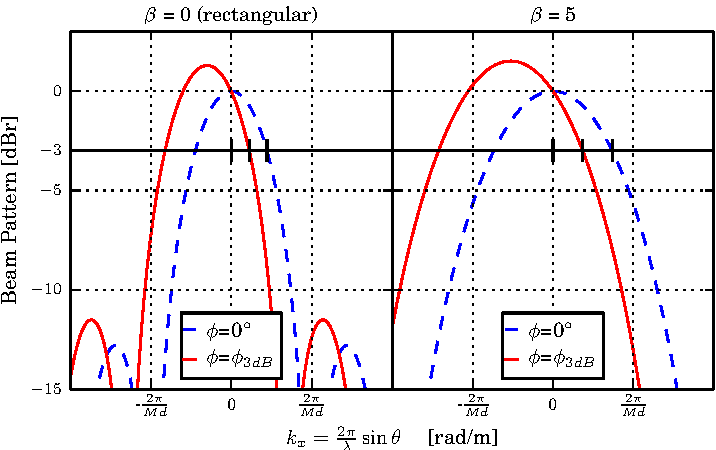
\includegraphics[width=\linewidth]{gfx/calc_kaiser_3dB.pdf}%
\caption{Each Kaiser window is steered in the interval $\phi=[0, \phi_{\text{-3dB}}(\beta)]$. The angle $\phi_{\text{-3dB}}(\beta)$ is the amount of steering needed for the steered response to have a -3dB crossing that is exactly half that of the unsteered window. With each window steered this way we expect the resolution gain to remain predictable and independent of $\beta$, and we also effectively constrain the white noise gain of the beamformer.}\label{windows_steering}
\end{figure}

\subsection{Steering}

\begin{align}
\w_{\beta,\phi} = \f_\beta\H\diag{(\a_\phi)}\\
\end{align}
%
where
%
\begin{align}
\a_\phi = \bmat{
1 \\
e^{-j\frac{md}{\lambda}\sin(\phi)} \\
\vdots\\
e^{-j\frac{(M-1)d}{\lambda}\sin(\phi)}
}
\end{align}


Before we apply the window to the sensor data, we normalize it to ensure unit gain in the direction of interest:
%
\begin{align}
\w = \frac{\vec f}{\f\T\1} \quad\quad\text{where}\quad\quad \f =
\bmat{
f_0 \\ \vdots \\ f_{M-1}                                                           
}
\end{align}
%
Note that the normalization factor $\f\T\1$ is the reciprocal of the window's coherent gain. Since the signal-to-noise gain is constant for a given window, this normalization also proportionally increases the  incoherent noise gain.

\begin{align}
\w = \frac{\a\f}{\f\T\a} = 
\end{align}


The steering is subject to an upper steering bound specified, which will be discussed next.


\subsection{Steering bounds}

There is an upper bound to the amount of steering we should apply to a window. Since each window's response is constrained to a unit gain in the look direction, each steered window's response is gained as shown in \Fig{windows_steering}. This increases the white noise gain and deteriorates the signal to noise ratio. To limit this we placing an upper bound to the steering, taking into account that a wide window can be allowed more steering than a narrow one.

We call the upper bound for steering $\phi_{\text{-3dB}}(\beta)$, and define it as the steering angle needed for the steered response to have a -3dB crossing that is exactly half that of the unsteered window. We numerically searched for the steering angle $\phi$ that fulfilled this criterion for a wide range of $\beta$-values. An explicit expression for was finally obtained with a third degree polynomial fit:
%
\begin{align}
\phi_\text{-3dB}(\beta) \approx -0.002894\beta^3 + 0.02451\beta^2 + -0.01308\beta + 0.2980
\end{align}
%
Any steering will be specified relative to this upper bound. With each window steered this way we expect the resolution gain to remain predictable and independent of $\beta$, and we also effectively constrain the white noise gain of the beamformer.

\subsection{Oversampling and steering}

Too much steering, beamformer becomes too agressive. Uncertainty in source amplitude grows.

\begin{itemize}
\item More steering -> more aggressive suppression of interference at the cost of boosted sidelobes / noise.
\item More steering -> Larger variations in amplitude of sources
\end{itemize}

Idea to steer within a fraction of the rectangular window's mainlobe. 

\begin{align*}
d = \frac{\pi\,\theta_\text{open}\,\lambda}{M\,d\,O_s}
\end{align*}

\begin{align}
\w[\beta, \phi] = \text{kaiser}(\beta) = \bmat{
1 \\
e^{-j\frac{md}{\lambda}\sin(\phi)} \\
\vdots\\
e^{-j\frac{(M-1)d}{\lambda}\sin(\phi)}
}
\end{align}

See section \ref{kaiser_windows}.


% Narrow ones:
% - Best coherent gain, lowest equivalent noise bandwidth, and most sensitive to steering meaning not needing to steer as much for some effect.
% 
% 
% Beamforming:
% - Maximize resolution
% - Minimize noise/error, both coherent and incoherent
% - Minimize signal cancellation
% 
% Gauss: Miminized time-bandwidth product
%   - 
%   
% Rectangular
%   - 
% Dolph-Cheb: Minimize mainlobe width given sidelobe suppression
% Kaiser: For a restricted energy and time duration, maximize energy in the band of frequencies W.
% 
% Adaptive windows perform best in detection of closely separated angles of significantly amplitudes.

% Adaptive beamformers usually compute the window coefficients by estimating and inverting a spatial covariance matrix. There are two inherent problems to this procedure. First, for improved estimation accuracy the data is either averaged in space or time, and the significance of the covariance matrix can be reduced using a regularisation parameter~\cite{Carl Inge}. These are all attempts to constrain the beamformer to ensure the window coefficience are not over-adapted to the data. Second, inverting the covariance matrix has a computational complexity of O($M^3$)~\cite{Carl Inge}. For larger arrays the computational burden becomes significant, and the question arises whether this processing power can be better utilised. 
% 
% 

% \section{Experimental Setup}
% 
% For the LCA to perform well it is important to let it have a diverse selection of windows to choose from. The question is how this selection should be With our ovarall goal being a reduction of computational complexity, it The choice of window function does not seem to matter. 
% 
% 
% 
% Using Kaiser windows as their extremal values areLimit our study to Kaiser windows
% 
% 
% 
% This selection is based on observations of the solutions found by the MV beamformer. We obtained good results in our experiments by letting the LCA beamformer select among 5 Kaiser windows with uniformly distributed $\beta$'s in the range $[0.05, 0.5]$ and a rectangular window. Each window was steered in 5 different directions, uniformly distributed within 80\% of the mainlobe width of the rectangular window, which is the most narrow. This adds to a total of 30 windows.
% 
% To make the choice of window less susceptible to pixel value uncertainties, the LCA beamformer was set to apply the most frequently selected window in an 11 pixel range region to the center pixel in that region. In physical terms, this is a region of approximately 20\,cm. The MV beamformer estimated the covariance matrix as described in~\cite{syn07} by averaging over 16 subarrays and 11 range pixels, and applying 3\% diagonal loading.


% Furthermore, the algorithm maps well to single-instruction-multiple-data (SIMD) hardware such as graphics processing units (GPUs). We show that even a modest amount of optimisation work has resulted in a factor 10 speed-up of this algorithm when implemented on a GPU as opposed to on a CPU.

\begin{figure*}[tbhp!]\centering%
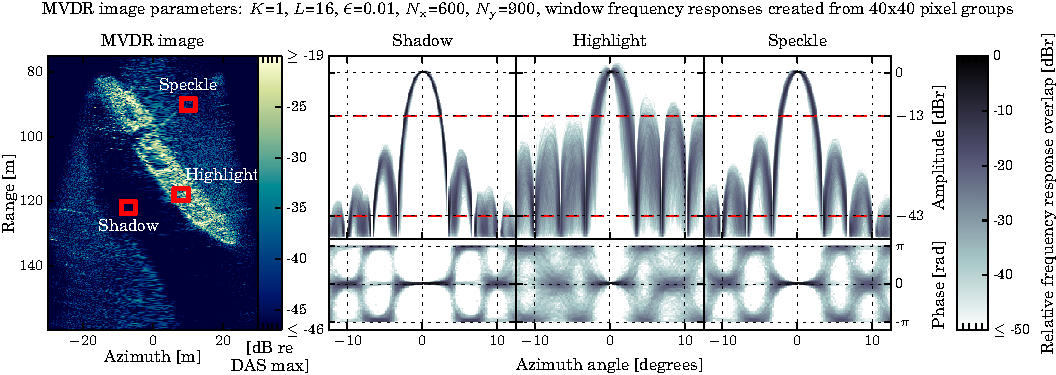
\includegraphics[width=\linewidth]{gfx/mvdr_selected_windows_holmengraa.pdf}%
\caption{Typical frequency responses for windows computed by a robust MVDR. The image is of the oiltanker Holmengraa, data collected from the 32 element HISAS1030 sonar with , operated in ssectorscan mode with an oversampling factor of ~10. The window responses was computed from 40x40 pixel groups in the shadow, highlight and speckle region. The dashed red lines at -13dB and -43dB marks the peak sidelobe level of a rectangular and Hamming window, respectively. Note how the responses are more or less symmetric, with very little steering in the shadow, moderate steering in speckle and steering within roughly 3dB in highlight. The phase varies mostly in highlight. Full opening angle. Parameters. }\label{mvdr_selected_windows}
\end{figure*}

\newpage

\section{Results and Discussion}

To test the performance of the MVDR and LCA beamformers, we have processed data aquired by the Kongsberg Maritime HUGIN AUV carrying their 32 element HISAS1030 sonar~\cite{Hansen2009}. It is a high resolution synthetic aperture sonar with array length 1.2\;m, 100\;kHz operating frequency, a bandwidth of 40\;kHz and transmits at a 25$^\circ$ opening angle.

Two different scenes will be presented. One of the 1500 dwt oiltanker wreck Holmengraa lying at a slanted seabed at 77\;m depth outside of Horten, Norway~\cite{holmengraa}. It measures 68\;m by 9\;m and fills most of the highlit sector. The other scene is of an iron cross connected to a an anchor (fig ???).

A quick summary of the results and the order they will be presented is as follows:

\begin{itemize}
\item \emph{Window function}. Frequency responses of typical windows chosen by MVDR in shadow, speckle and highlight regions in an image is shown in \Fig{mvdr_selected_windows}. The responses tend to be symmetric, minimally steered and have slightly varying mainlobe width and sidelobe suppression. We use Kaiser windows to mimic these responses.
\item \emph{Window parameters}. The Kaiser window parameter $\beta$ adjusts the compromise between resolution and sidelobe suppression. At $\beta=0$ it yields a rectangular window, and at and $\phi$ controls the amount of steering.. $\beta=0$ ) and a gaussian curve (
\end{itemize}

The following sections with expand and discuss these results further.

\subsection{Window function}

Assuming that a robust MVDR computes the optimal windows in the minimum variance sense, it makes sense to study them. For this we selected a scene of the oil tanker wreck Holmengraa, which lies at a slanted seabed at nearly 100m\;depth. A sectorscan image of a single ping of data collected by the HISAS1030 syntetic aperture sonar is shown in \Fig{mvdr_selected_windows}, along with the window responses MVDR typically chooses in shadow, speckle and highlight regions in this image. A fairly agressive yet stable set of parameters for MVDR where used; subarray size $L=16$, temporal averaging of $K=1$, and $d=1\%$ of diagonal loading.

While MVDR is free to choose non-symmetric windows, we can observe from \Fig{mvdr_selected_windows} that it prefers symmetric ones. In shadow and speckle the windows are fully symmetric, while in highlight the windows are approximately symmetric within the opening angle of the sonar. 


\subsection{Window parameters}

The Kaiser window parameter $\beta$ adjusts the compromise between resolution and sidelobe suppression, and $\phi$ controls the amount of steering. At $\beta=0$ it becomes a rectangular window, and at larger values it approaches a gaussian curve. Typical values are in the range $\beta\in[0,10]$.

$\phi$ controls the amount of steering. 

The Kaiser window parameter $\beta$ adjusts the compromise between resolution and sidelobe suppression. At $\beta=0$ it yields a rectangular window, and at and $\phi$ controls the amount of steering.. $\beta=0$ ) and a gaussian curve (


\begin{figure*}[tbhp!]%\centering%
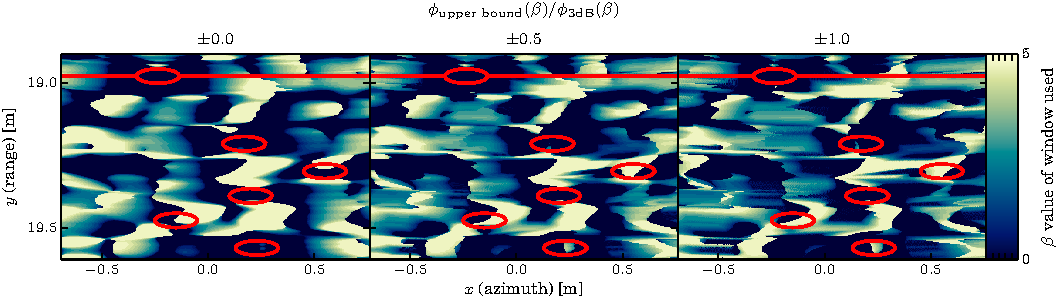
\includegraphics[width=\textwidth]{gfx/oversampling_mosaic_bounds_lca_windows_beta.pdf}%
\caption{Window parameter boundaries. Oversampled image, 19x20 windows.}\label{oversampling_mosaic_bounds}
\end{figure*}

\newpage
\begin{figure*}[tbhp!]%\centering%
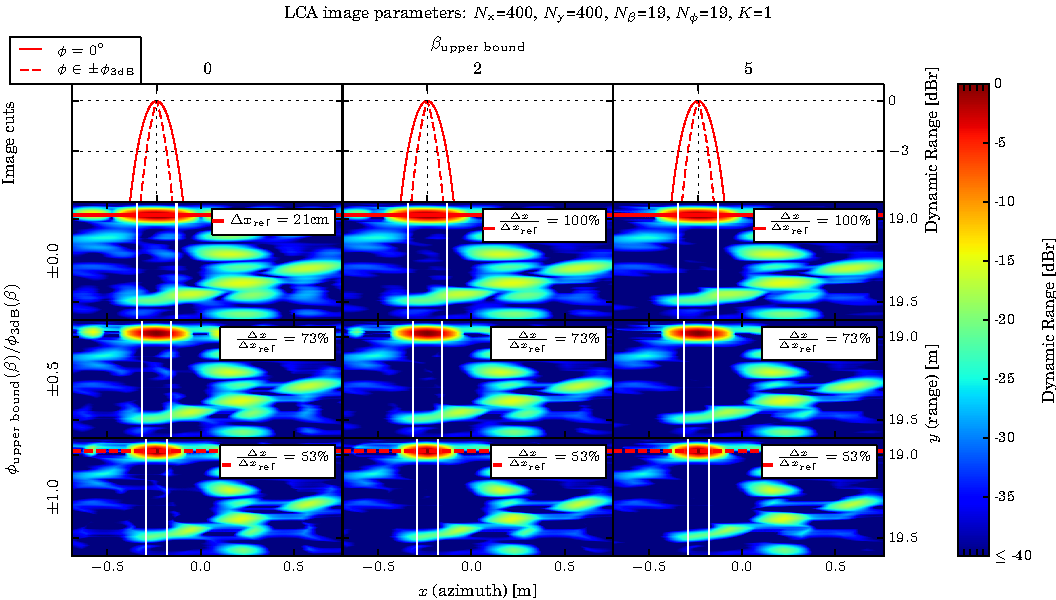
\includegraphics[width=\textwidth]{gfx/oversampling_mosaic_bounds.pdf}%
\caption{Window parameter boundaries. LCA images using an oversampled image and a relatively large window database with $N_\beta=20$ window types, each steered $N_\phi=19$. }\label{oversampling_mosaic_bounds_beta}
\end{figure*}


Variables of interest:

\begin{itemize}
\item Window function. Mostly symmetrical, in particular in shadow and for the most part in speckle. In highlight regions more varying.
\item Mainlobe width. Wide in shadows, narrow in detailed regions. Adding windows in between these extremal values.
\item Steering. No steering in shadows, slight steering in speckle and no steering in highlight. Steering more than the -3dB width of the window function has no effect.
\item Oversampling. From our observations one should have at least twice the number of beams as channels. Image is more visually pleasing and appears more detailed up to 8M.
\end{itemize}
\begin{table}[!b]\centering%\normalsize
\begin{tabular}[c]{l c c c}\hline
\rowcolor{tabBlue} & \bf Highlight & \bf Shadow & \bf Speckle  \\\hline
Symmetry             & Moderate  & High   & High \\
Mainlobe width       & Narrow    & Wide   & Moderate \\
Sidelobe suppression & Low       & High   & Moderate \\
Steering             & Low       & Up to -3dB width & Moderate \\
Oversampling         & 2x-8x     & 2x-8x  & 2x-8x
\end{tabular}
\caption{Summary}\label{tab:summary}
\end{table}%



oversampled 10 times in azimuth~\cite{Asen2014}.

\newpage


% the performance of the LCA beamformer is surprisingly similar regardless of what windows it is allowed to choose from.

\newpage

What's wrong here? 

\begin{figure*}[tbhp!]%\centering%
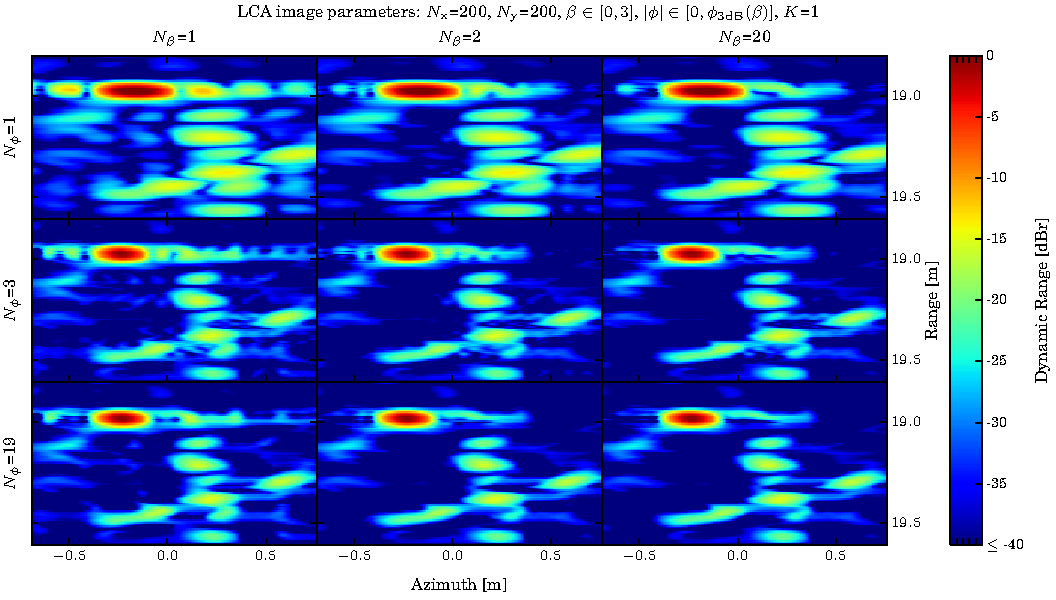
\includegraphics[width=\textwidth]{gfx/oversampling_mosaic.pdf}%
\caption{Window parameter boundaries. Oversampled image, 19x20 windows.}\label{oversampling_mosaic}
\end{figure*}


\begin{itemize}
\item Oversampling tests. Both Holmengraa and cross.
\item Mosaic indicating the number of windows needed.
\item 
\end{itemize}



% \begin{table}[!b]\centering%\normalsize
% \begin{tabular}[c]{l r r r@{}  l}\hline
% \rowcolor{tabBlue} & \multicolumn{1}{>{\columncolor{tabBlue}}c}{\bf B$_\text{arith}$} & \multicolumn{1}{>{\columncolor{tabBlue}}c}{\bf B$_\text{mem}$} & \multicolumn{2}{>{\columncolor{tabBlue}}c}{\bf B$_\text{mem}$/B$_\text{arith}$} \\\hline
% Arithmetic & 1.03 Tflop/s & & &\\
% Global memory & & 36 Gfloats/s & \hspace{30pt} 1 &:30 \\
% Shared memory & & 257 Gfloats/s & 1 &:4 \\
% Registers & & $>$1.5 Tfloats/s & $>$3 &:2~\cite{Vasilyy}
% \end{tabular}
% \caption{Nvidia Quadro 6000: Memory throughput, $B_{\lowercase{\text{mem}}}$, compared to arithmetic throughput, $B_\text{arith}$.}\label{throughputs}
% \end{table}%

\newcommand\cc[1]{\multicolumn{1}{>{\columncolor{tabBlue}}c}{\bf #1}}
\begin{table}[!b]\centering%\normalsize
\begin{tabular}[c]{l r r r@{}  r r r}\hline
\rowcolor{tabBlue} & \cc{Resolution} & \cc{S} & \cc{$\beta$} & \cc{$\varphi^*$} &  \cc{N$_\beta$} & \cc{N$_\varphi$} \\\hline
& 50\%  & 28 & [0,3] & \hspace{.15cm} 50\% & 2 & 3 \\
& 50\%  & 28 & [0,6] & \hspace{.15cm} 50\% & 2 & 3 \\
& 50\%  & 28 & [0,9] & \hspace{.15cm} 50\% & 2 & 3 \\
& 100\% & 32 &  &:30 \\
& 150\% & 32 & 1 &:4\\
\end{tabular}\\
* Steering is relative to the -3dB width of the window being applied.
\caption{Qualitative study}\label{parameter_study}
\end{table}%


% The simulations contained a few highlighted cylindric regions with 2\,m diameter and a constant intensity 15.4\,dB over the average speckle level. We focused on an object centered at 41\,m range and -3 degrees azimuth angle. The images produced by the LCA, MV and unweighted DAS for a single speckle realisation and a mean image of all 100 realisations are shown in \Fig{speckle}. Each image was normalised by their respective speckle level, and the dynamic range was clamped at \{-30,~15\}\,dB. The physical extent of the of the simulated object was superimposed for reference. %\ref{saf09}
% 
% In \Fig{speckle} we observe that both the adaptive beamformers produce images with a more clearly defined shadow. The edges are sharper and the shadow more distinct. This is because the adaptive beamformers have better sidelobe suppression, and thus allow less signal energy to leak from the speckle region into the shadow region. The same effects can also be observed laterally around the highlight region of the mean image; DAS is more prone to smear energy into the speckle region than the adaptive beamformers are.
% 
% \Fig{cutmean} displays two lateral cuts in the mean image, one through the highlight at 41.1\,m range and one through the shadow at 44.5\,m range. Each cut was computed as the mean of a 40\,cm range band centered at the respective ranges. The transition region between highlight and shadow is shortest for the LCA, which is advantageous since it results in a more accurate representation of the object size. The slightly inferior performance of the MV beamformer is due to the subarray averaging, which makes the effective array smaller~\cite{syn07}.
% 
% By studying the LCA performance on the 100 speckle realisations, we found the choice of window to be highly dependent on the phenomena being imaged. In speckle regions LCA favored narrow spatial responses with minor steering, while wide and fully steered responses were often selected in shadow regions. There was also a clear distinction between the responses selected in sidelobe regions and in speckle regions.
% 
% % \Fig{hist} illustrates how often a particular window is chosen in general. There are 10 $\phi$'s for each of the 10 $\beta$'s. The first 10 values are rectangular windows. Value 5 is a non-steered rectangular window, and we see that this is most frequently selected. At higher steering angles the windows are rarely selected, and thus we might get better results by tightening our steering boundaries. At value 15 we find inverted Kaiser windows with $\beta = 0.05$, and then $\beta$ is increased in increments of 0.505 for every 10th value. At value 65 the $\beta$ value is 2.025, and these and the remaining windows are hardly selected.
% 
% A sidescan image of the 1500 dwt oil tanker wreck Holmengraa is shown in \Fig{holmengraa}. It is about 68\,m long and 9\,m wide, and lies on a slanted seabed at 77\,m depth~\cite{holmengraa}. The sidescan image was created using data from the HISAS 1030 sonar, which is rather unsuited for this purpose because of its large opening angle. This, and the fact that the wreck was imaged at a range of about 105\,m makes the image quality poor, but sufficient to compare our beamformers. 
% 
% In the Holmengraa image we note again that the LCA produces a cleaner shadow and better edge definition. The MV method performed almost identically to LCA in this case, and was omitted.


\section{Conclusion}

The LCA method performs similar to the MV method, but at a fraction of the computational cost. The key to achieve this success lies in the design of the window set. Windows that yield vagely steered narrow responses are preferred in speckle regions, while wide and steered responses are typically preferred in highlight and shadow regions. A window set of 6 different responses each steered in 5 different directions proved sufficient in our experiment to match the performance of the MV beamformer.

The tendency of the LCA to perform similarly to the MV beamformer seems to indicate that a full solution space is rarely needed in real world scenarios. 


\subsection{Summary and order of results}

In short, our findings regarding the optimal window types for LCA is as follows:

\begin{itemize}
\item \emph{Window function} should be symmetric, . Studying typical MVDR responses for shadow, speckle and highlight regions, we believe it to be insignificant
\item \emph{Window parameters}. 
\end{itemize}

The following sections with expand and discuss these results further.

\section{Introduction}


% \begin{itemize}
% \item Sell it!
% \item As briefly as possible, introduce beamforming.
% \item Adaptive beamformer's potential lies in its ability to suppress interference power
% \item Why adaptive beamformers struggle in active sonar systems. Correlated noise, robustification kills the adaptive potential. Quite computationally intensive. Constraints must be applied in one way or another - parameters must be tuned.
% \begin{itemize}
% \item Noise and signal is correlated. Spatial averaging required. 
% \item Increases variance of speckle (not only in active systems?), spatial compunting \cite{Vignon2009} (US) or time averaging?. Subarray averaging applied here \cite{Synnevag2007} (US) \todo{Is it bad to mix ultrasound/ sonar refs?}
% \end{itemize}
% \item LCA is like DAS, only we test several windows and choose the one that yield the lowest beamformer output power. Ultrasound \cite{Synnevag2008}, active sonar \cite{Buskenes2011}\cite{Blomberg2011}\cite{Blomberg2012}\todo{who was that guy in the 80ties?}
% \item Outline: 
% \begin{itemize}
% \item Methods.
% \item See what happens to Capon's response %\cite{Synnevag2007}  when means for robustification are added.
% \item Setup the window set for LCA to match this.
% \item Notice that the LCA performs like Capon, even with a small window database.
% \item Start with Kaiser, see that other window functions also work well.
% \end{itemize}
% \end{itemize}
% \todopar{Out of the blue idea: Weigh CF with LCA? This guy did it with MVDR \cite{Wang2009}. Probably you know already... Okay, back on track.}


\section{Methods}

\todopar{Threw some formulas in to get a feel of them}

\begin{align}
z[n] = \sumb{m=0}{M-1} w_m[n]^*x_m[n-\Delta_m] = \w\H[n]\Xd[n]
\end{align}
where
\begin{align}
\w[n] = \bmat{w_0[n]\\w_1[n]\\\vdots\\w_{M-1}[n]} \quad \text{and} \quad\Xd[n] = \bmat{x_0[n]\\x_1[n]\\\vdots\\x_{M-1}[n]}.
\end{align}

Minimum variance distortionless resonse \cite{Capon1969}
\begin{align}
\underset{\w[n]}{\argmin}\, E\{ |z[n]|^2 \} = \underset{\w[n]}{\argmin}\, \w\H[n]\R[n]\w[n], 
\end{align}
subject to
\begin{align}
\w\H[n]\a = 1,
\end{align}
where
\begin{align}
\R[n] = E\{ \x\x\H \}.
\end{align}


\section{Results}

% \begin{figure}[!t]\centering
% % \includegraphics[width=2.5in]{}
% \caption{Simulation Results}
% \label{fig_sim}
% \end{figure}

See end of document...
% \begin{figure*}[!t]
% \centerline{\subfloat[Case I]\includegraphics[width=2.5in]{subfigcase1}%
% \label{fig_first_case}}
% \hfil
% \subfloat[Case II]{\includegraphics[width=2.5in]{subfigcase2}%
% \label{fig_second_case}}}
% \caption{Simulation results}
% \label{fig_sim}
% \end{figure*}



\section{Conclusion}

\begin{itemize}
\item Something similar to the abstract.
\end{itemize}


% \ \\
% \IEEEPARstart{T}{o} form images from a modern phased array sonar system the received wavefield is usually recorded, and then postprocessed by a digital beamformer. The beamformer applies delays and weights to the sensor channels, the beamformer adjusts the arrays spatial response to focus at one pixel at a time.  such that signals emanating from regions of interest add constructively, while ensuring that noise and interference from other angles do not. 
% 
% The imaging capabilities of a modern phased array sonar system depend on physical attributes such element response and array geometry, the transmitted signal, as well as the beamforming method being used on transmission and reception. Beamforming is the concept of applying delays and weights to the sensors channels to steer the arrays response to points of interest. 

% 
% 
% Outline:
% \begin{itemize}
% \item Capon's resonse when applying robustification
% \item Choice of window functions makes little difference.
% \item Steering and mainlobewidths have outer bounds.
% \item Beamspace?
% \item Chosen window plots - what may they tell us? Variance intensity values when using various windows.
% \item Assymmetric windows?
% \end{itemize}
% 
% 
% \begin{align}
% z[n] = \sumb{m=0}{M-1} w_m[n]^*x_m[n-\Delta_m] = \w\H[n]\x[n-\Delta_m]
% \end{align}
% 
% 
% \section{Methods}
% 
% Basically, we are working with a practical implementation of the Capon beamformer that computes a set of weights $\vec w$ for every single sample $n$ by solving:
% \begin{gather*}
% \vec w[n] = \frac{\hat{\mat R}\,\!^{-1}[n]\vec a}{\vec a\H\hat{\mat R}\,\!^{-1}[n]\vec a} = \frac{\text{\raisebox{1.9pt}{$\vec\chi$}}[n]}{\vec a\H\text{\raisebox{1.9pt}{$\vec\chi$}}[n]}
% \end{gather*}%
% where
% % \newcommand\X{\text{\raisebox{2pt}{$\vec\chi$}}}
% \begin{gather*}
% \text{\raisebox{1.9pt}{$\vec\chi$}} = \hat{\mat R}\,\!^{-1}\vec a \qquad\qquad\text{is the solution to}\qquad\qquad \hat{\mat R}\text{\raisebox{1.9pt}{$\vec\chi$}} = \vec a.
% \end{gather*}

% 
% , and maximum suppression of while ensuring that the beamformer digitally  before each of the pixels are estimated one at a time. The resolution and contrast of such a system will depend on the systems spatial response, which ideally should be narrow  be very sharp in the desired direction its ability to achieve  fundamental principle of forming a sonar image is to record the received wavefield, 
% 
% image quality of a phased array sonar imaging systems depend on  the choice of weights to apply to each of the sensors are crucial. 
% 
% A modern phased array imaging system may be thought of as a spatial filter. To achieve the best possible performance, the 
% 
% resolution and contrast 
% 
% Adaptive beamformers have only recently been introduced in active sonar imaging. For a while they were considered unsuited for this purpose because the backscattered signal is largely correlated with the 
% 
% 
% 

%\begin{figure}[!t]
%\centering
%\includegraphics[width=2.5in]{myfigure}
% where an .eps filename suffix will be assumed under latex, 
% and a .pdf suffix will be assumed for pdflatex; or what has been declared
% via \DeclareGraphicsExtensions.
%\caption{Simulation Results}
%\label{fig_sim}
%\end{figure}


% An example of a double column floating figure using two subfigures.
% (The subfig.sty package must be loaded for this to work.)
% The subfigure \label commands are set within each subfloat command, the
% \label for the overall figure must come after \caption.
% \hfil must be used as a separator to get equal spacing.
% The subfigure.sty package works much the same way, except \subfigure is
% used instead of \subfloat.
%
% \begin{figure*}[!t]
% \centerline{\subfloat[Case I]\includegraphics[width=2.5in]{subfigcase1}%
% \label{fig_first_case}}
% \hfil
% \subfloat[Case II]{\includegraphics[width=2.5in]{subfigcase2}%
% \label{fig_second_case}}}
% \caption{Simulation results}
% \label{fig_sim}
% \end{figure*}
%
% Note that often IEEE papers with subfigures do not employ subfigure
% captions (using the optional argument to \subfloat), but instead will
% reference/describe all of them (a), (b), etc., within the main caption.


% An example of a floating table. Note that, for IEEE style tables, the 
% \caption command should come BEFORE the table. Table text will default to
% \footnotesize as IEEE normally uses this smaller font for tables.
% The \label must come after \caption as always.
%
%\begin{table}[!t]
%% increase table row spacing, adjust to taste
%\renewcommand{\arraystretch}{1.3}
% if using array.sty, it might be a good idea to tweak the value of
% \extrarowheight as needed to properly center the text within the cells
%\caption{An Example of a Table}
%\label{table_example}
%\centering
%% Some packages, such as MDW tools, offer better commands for making tables
%% than the plain LaTeX2e tabular which is used here.
%\begin{tabular}{|c||c|}
%\hline
%One & Two\\
%\hline
%Three & Four\\
%\hline
%\end{tabular}
%\end{table}


% Note that IEEE does not put floats in the very first column - or typically
% anywhere on the first page for that matter. Also, in-text middle ("here")
% positioning is not used. Most IEEE journals use top floats exclusively.
% However, Computer Society journals sometimes do use bottom floats - bear
% this in mind when choosing appropriate optional arguments for the
% figure/table environments.
% Note that, LaTeX2e, unlike IEEE journals, places footnotes above bottom
% floats. This can be corrected via the \fnbelowfloat command of the
% stfloats package.



\section{Conclusion}
The conclusion goes here.


We limit our study to the use of variations of the parametric Kaiser-Harris window, since we observed neglible performance difference to using this function or any of the common trigonometric ones. The Kaiser windows are easy to compute, is fairly insensitive to coefficient inaccuracies, and can create windows with shapes spanning from rectangular to Gaussian.




% if have a single appendix:
%\appendix[Proof of the Zonklar Equations]
% or
%\appendix  % for no appendix heading
% do not use \section anymore after \appendix, only \section*
% is possibly needed

% use appendices with more than one appendix
% then use \section to start each appendix
% you must declare a \section before using any
% \subsection or using \label (\appendices by itself
% starts a section numbered zero.)
%

%%%%%%%%%%%%%%%%%%                              ~~~~~~~~~~~~~~~~~~~~~~~~~~~~~~~~~~~~~~~~~~~~~~~~~~
% DOCUMENT APPENDICES %
%%%%%%%%%%%%%%%%%%                              ~~~~~~~~~~~~~~~~~~~~~~~~~~~~~~~~~~~~~~~~~~~~~~~~~~

\appendices



% use section* for acknowledgement
\ifCLASSOPTIONcompsoc
  \section*{Acknowledgments}
\else
  \section*{Acknowledgment}
\fi


The authors would like to thank...


% Can use something like this to put references on a page
% by themselves when using endfloat and the captionsoff option.
\ifCLASSOPTIONcaptionsoff
  \newpage
\fi



\bibliographystyle{IEEEtran}
\bibliography{references}
% 
% 
% 
\begin{IEEEbiography}[{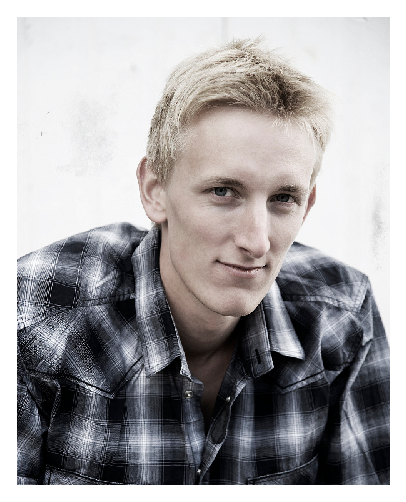
\includegraphics[width=1in,height=1.25in,clip,keepaspectratio]{bio/jo_inge.eps}}]{Jo Inge Buskenes}
received the B.Sc. degree in electrical engineering from Gj\o{}vik College University, Norway, in 2007, and the M.Sc. degree in instrumentation for particle physics from the University of Oslo, Norway, in 2010. He is currently pursuing the Ph.D. degree in image reconstruction and technology at the University of Oslo.

His industry experience includes the European Organization for Nuclear Research (CERN), Geneva, Switzerland (2007-2008), and the Norwegian Defence Research Establishment, Kjeller, Norway (2009). He has lectured in digital signal processing at the Gj\o{}vik College University (2009), and at the University of Oslo (2010-2013). His research interests include adaptive beamforming, digital image reconstruction, high performance computing, intelligent detector design and open source software.
\end{IEEEbiography}
% % 
\begin{IEEEbiography}[{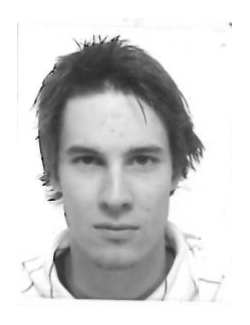
\includegraphics[width=1in,height=1.25in,clip,keepaspectratio]{bio/jon_petter.eps}}]{Jon Petter \AA{}sen}
(S'12) was born in Porsgrunn, Norway in 1986. He received the B.Sc. and M.Sc. degree in computer science from the University of Oslo, Norway, in 2010. He is currently pursuing his Ph.D. degree in medical ultrasound technology at the Norwegian University of Science and Technology (NTNU) Medical Imaging Lab (MI-Lab), Trondheim, Norway. His research interests include adaptive ultrasound processing techniques and acceleration of ultrasound algorithms using Graphics Processing Units (GPUs). 
\end{IEEEbiography}
% % 
\begin{IEEEbiography}[{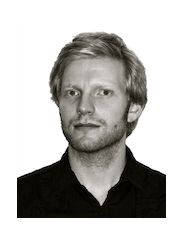
\includegraphics[width=1in,height=1.25in,clip,keepaspectratio]{bio/carl-inge.eps}}]{Carl-Inge Colombo Nilsen}
(S'06-M'10) received the M.Sc. and Ph.d. degrees in computer science from the University of Oslo, Norway, in 2005 and 2010. He is currently working at the University of Oslo as a postdoctoral research fellow. His research interests include signal and array processing for ultrasound imaging and other acoustical applications.
\end{IEEEbiography}
% 
\begin{IEEEbiography}[{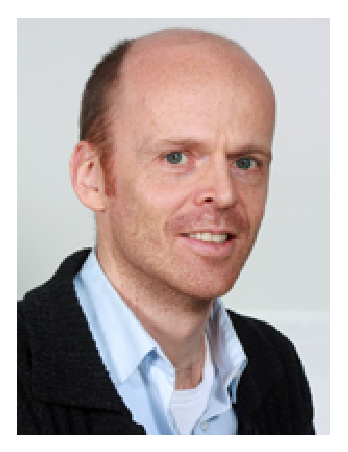
\includegraphics[width=1in,height=1.25in,clip,keepaspectratio]{bio/andreas.eps}}]{Andreas Austeng}
was born in Oslo, Norway, in 1970. He received the M.Sc. degree in physics in 1996 and the Ph.D. degree in computer science in 2001, both from the University of Oslo. Since 2001, he has been working at the Department of Informatics, University of Oslo, first as a postdoctoral research fellow and currently as an associate professor. His research interests include signal and array processing for acoustical imaging.
\end{IEEEbiography}

\vfill 


\end{document}


